\section{Para-real method}
	
Para-real method is a parallel-in-time integration method which was introduced in 2001 by Lions, Maday and Turinici~\cite{partie2_ref1}. Parareal computes the numerical solution for multiple time steps in parallel and it is categorized as a parallel-across-the-steps method.

\subsection{Explanation}

As for the previous methods, we consider an initial value problem of the form \\
\begin{minipage}{\linewidth}
	\centering
	$\left\{\begin{aligned}
		X'&=f(t,X), \qquad t_0\le t\le T, \\
		X(t_0)&=X_0.
	\end{aligned}\right.$ \\
\end{minipage} \\

\subsubsection{Time decomposition}

\noindent Parareal method needs a decomposition of the time interval $[t_0,T]$ into $P$ slices $[t_j,t_{j+1}]$ with  $j\in\{0,\dots,P-1\}$, where $P$ is the number of process units. As we want to parallelize the algorithm, each time slice is assigned to one process. \\
We denote by $F$ an integrator which is of high accuracy and $G$ which is of low accuracy. Also, $F$ will be very expensive in terms of calculation but very accurate, and $G$ will be very cheap but very imprecise. We denote by $\Delta t_F$ the time step and by $\Delta t_G$ the coarse time step. To have the right number of points in total (i.e. the sum of the number of points of each interval is equal to the number of points between $t_0$ and $T$), we are not going to cut the interval in equal parts. However, the $t_j$ will have to be multiples of $\Delta t_G$ (we will choose the multiple of $\Delta t_G$ closest to $t$ which cuts our interval in equal parts).
For example, taking $P=3$ processes, $\Delta t_G=0.1$ and the interval from $t_0=0$ to $T=2$, our exact $t_j\in\{0,\;0.666,\;1.333,\;2\}$ which we will be approximated  by $\{0,\;0.7,\;1.3,\;2\}$. We will also suppose that the coarse time step $\Delta t_G$ is a multiple of the fine time step $\Delta t_F$. If this was not the case, a simple way to avoid the problems related to the number of points could be an interpolation with $t_j^G\in[t_i^F,t_{i+1}^F]$

\subsubsection{Principle of parareal method}
\label{section parareal method}

\noindent We denote by $U_j^k$, $j\in\{0,\dots,P\}$ the initial point at time $t_j$ and at iteration $k$. We also denote $F(U_{j-1}^k)$, $j\in\{1,\dots,P\}$ the result of the fine integrator between $t_{j-1}$ and $t_j$ which starts from the initial point $U_{j-1}^k$ at iteration $k$ and respectively $G(U_{j-1}^k)$, $j\in\{1,\dots,P\}$ the result of the coarse integrator between $t_{j-1}$ and $t_j$ which starts from the initial point $U_{j-1}^k$ at iteration $k$. Then, a series of steps (\textit{see Figure \ref{parareal}}) is performed until the solution of the system converges. \\

\noindent At iteration $k=0$ :
\begin{enumerate}[label=\textbullet]	
	\item Step 1 (\textit{see \ref{parareal:1}}) : At iteration $k=0$, we have an initial point $U_0^0=X_0$.
	\item Step 2 (\textit{see \ref{parareal:2}}) : We start by applying the function $G$ on all intervals $[t_j,t_{j+1}]$ and we denote by $U_j^0=G(U_{j-1}^0)$ the values of $G$ at $t_j$. \\
	Note that this part of the method must be done sequentially because if we parallelize the task, the process $j$ should wait until the process $j-1$ has finished before starting.
	\item Step 3 (\textit{see \ref{parareal:3}}) : We can then calculate from each $U_j^0$ the fine solution between $t_j$ and $t_{j+1}$ : $F(U_j^0)$. This is an operation that must be parallelized.
\end{enumerate}

\noindent At iteration $k=1$ :
\begin{enumerate}[label=\textbullet]	
	\item Step 4 (\textit{see \ref{parareal:4}}) : We can then continue to iteration $k=1$ where we need the values $G(U_j^0)$ and $F(U_j^0)$ calculated at the previous iteration ($k=0$). \\
	We will also keep the initial point at time $t_0$ : $U_0^1=U_0^0$.
	\item Step 5 (\textit{see \ref{parareal:5}}) : We can then calculate $G(U_0^1)$ which allows us to obtain the point $U_1^1$ by the following formula:
	$$U_j^1=G(U_{j-1}^1)+(F(U_{j-1}^0)-G(U_{j-1}^0)).$$
	Note that due to $U_0^1=U_0^0$, we have $G(U_0^1)=G(U_0^0)$ and therefore $U_1^1=F(U_0^0)$ \\
	We then compute in the same way the following $G(U_j^1)$ and the associated $U_{j+1}^1$ points. This step can be done sequentially for the same reason as in step 2.
	\item Step 6 (\textit{see \ref{parareal:6}}) : We can then calculate from each $U_j^1$ the fine solution between $t_j$ and $t_{j+1}$ : $F(U_j^1)$. This is an operation that must be parallelized. \\
	Note that due to $U_0^1=U_0^0$, we also have $F(U_0^1)=F(U_0^0)$.
\end{enumerate}

\noindent Then we repeat steps 3 to 6 until $U_j^k-U_j^{k-1}\rightarrow 0 \quad \forall j\in\{0,\dots,P-1\}$. \\
We have at iteration $k$:
$$U_j^k=G(U_{j-1}^k)+(F(U_{j-1}^{k-1})-G(U_{j-1}^{k-1}))$$

\noindent \underline{\textit{Remarks :}} At iteration k.
\begin{itemize}[label=-]
	\item We have : $\qquad U_0^k=U_0^0=X_0 \quad \forall k$.
	\item Note that the first 3 steps are always done because there can't be convergence with only one value. So, for example, if we take only one process and we apply the parareal method, we will have at the first iteration ($k=0$) only one initial point $U_0^0=X_0$ and we will compute the fine and coarse solution only on this point. We can then go to the next iteration, which will be exactly the same, and the algorithm will stop immediately. Indeed, there will be convergence between $U_0^0$ and $U_0^1$ (because they are equal), moreover there is obviously convergence between the 2 solutions. However, there is still one extra iteration ($k=1$) and the computation of the coarse solution is also useless because it is not used to update the other initial points due to the fact that there is only one.
	\item We can also notice that the calculations which are done on the last interval $[t_{P-1},t_P]$ are not used because the points $U_P^k$ are not useful for the method. On this interval, we could then compute the fine solution only if there is convergence.
\end{itemize}

\newpage

\noindent The following figure (Figure \ref{parareal}) illustrates the previous steps :

\begin{figure}[h]
	\captionsubfigure
	\fbox{
		\centering \qquad
		\begin{minipage}[c]{\linewidth}
			\begin{subfigure}[t]{.30\linewidth}       
				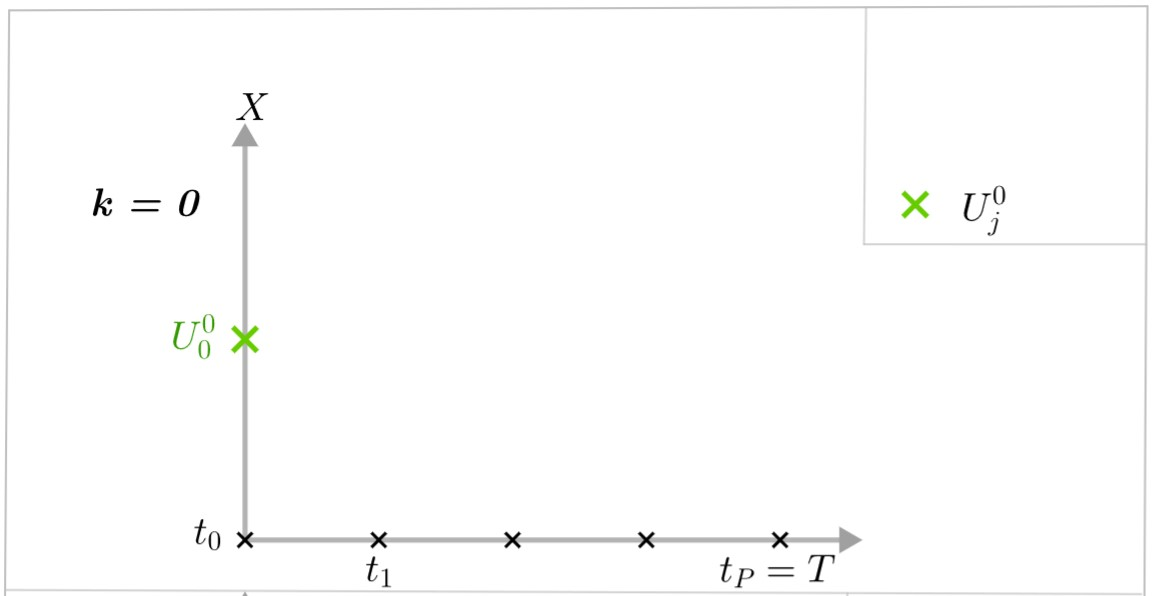
\includegraphics[width=\linewidth]{"images/parareal/parareal_1.jpg"}
				\captionof{figure}{ : Step 1}
				\label{parareal:1}
			\end{subfigure} 
			\begin{subfigure}[t]{.30\linewidth}       
				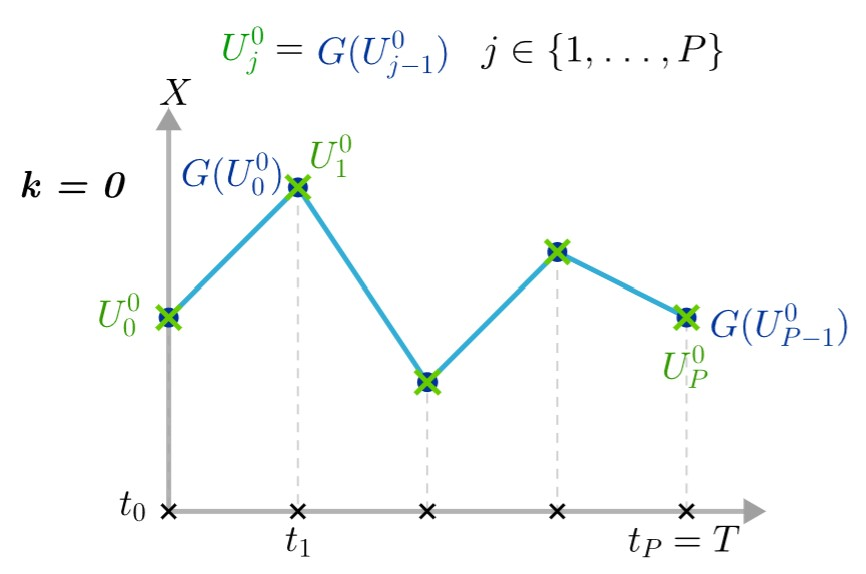
\includegraphics[width=\linewidth]{"images/parareal/parareal_2.jpg"}
				\captionof{figure}{ : Step 2}
				\label{parareal:2}
			\end{subfigure} 
			\begin{subfigure}[t]{.30\linewidth}       
				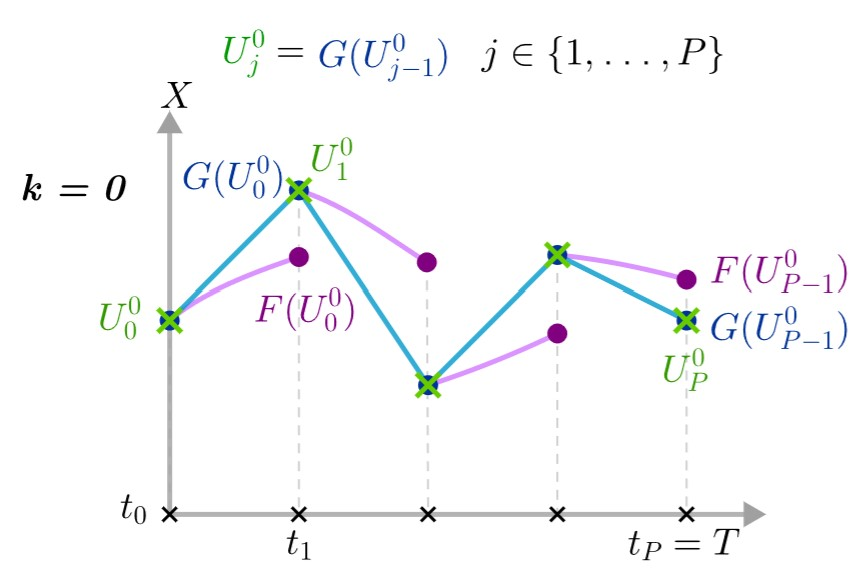
\includegraphics[width=\linewidth]{"images/parareal/parareal_3.jpg"}
				\captionof{figure}{ : Step 3}
				\label{parareal:3}
			\end{subfigure} 
			
			\begin{subfigure}[t]{.30\linewidth}       
				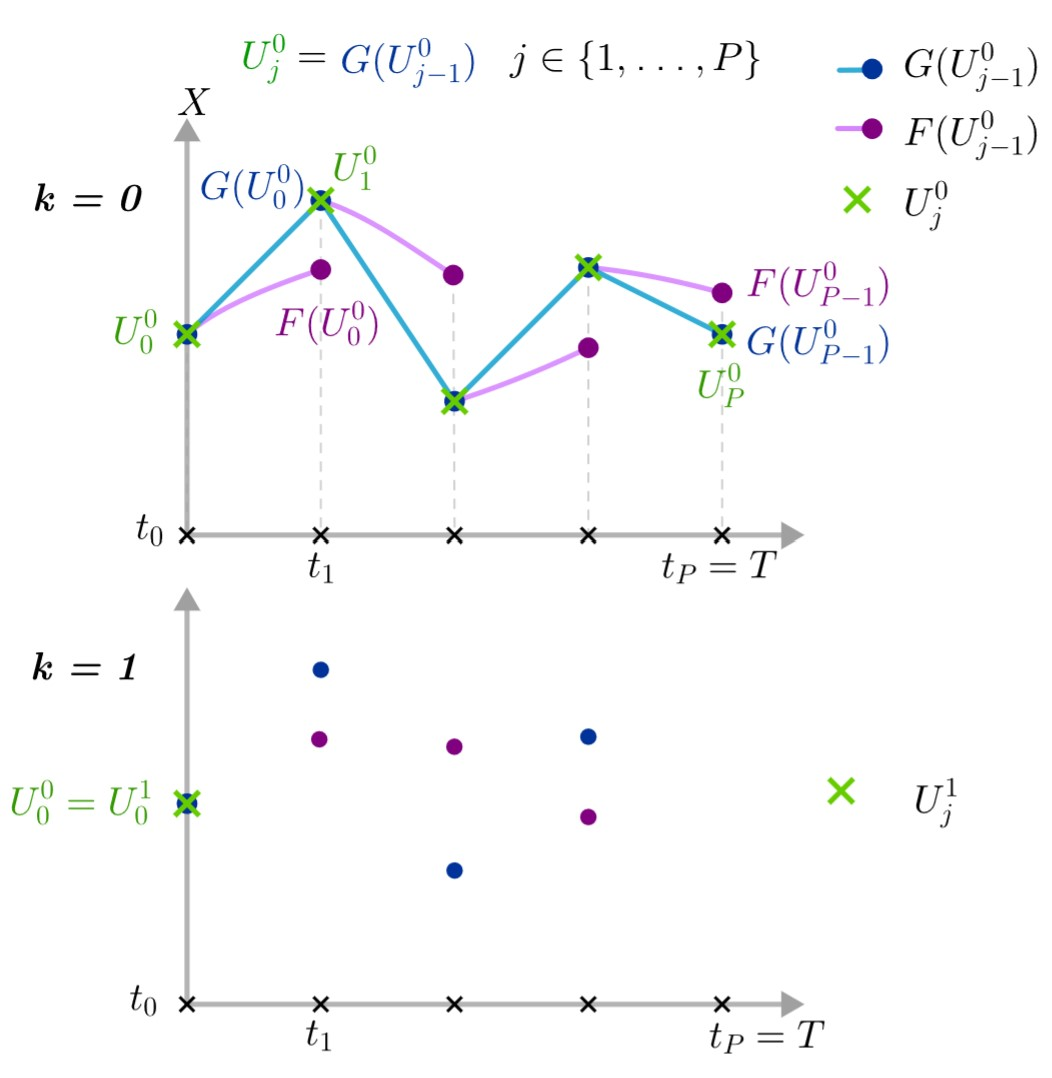
\includegraphics[width=\linewidth]{"images/parareal/parareal_4.jpg"}
				\captionof{figure}{ : Step 4}
				\label{parareal:4}
			\end{subfigure} 
			\begin{subfigure}[t]{.30\linewidth}  
				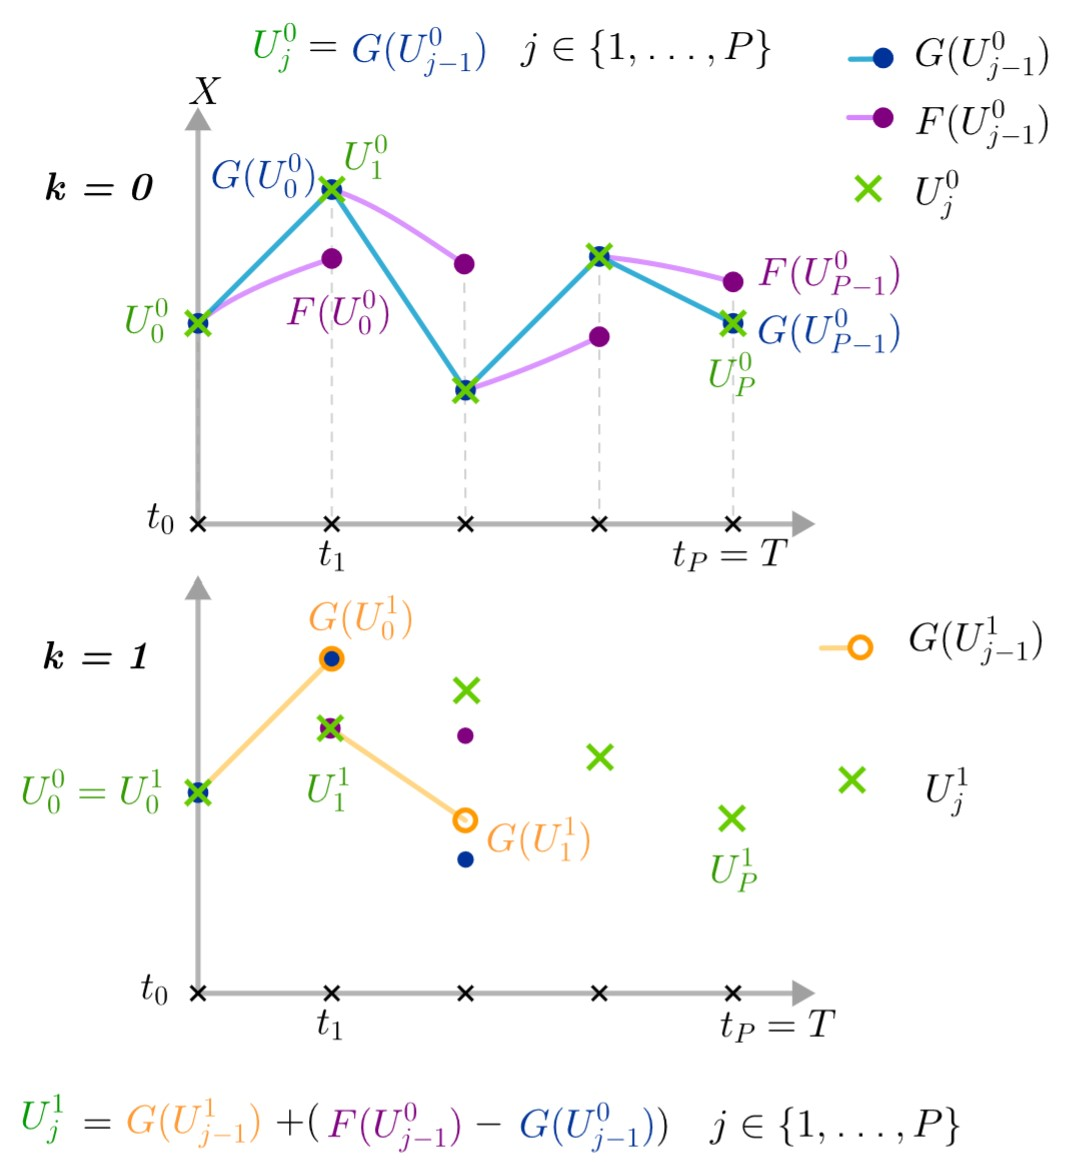
\includegraphics[width=\linewidth]{"images/parareal/parareal_5.jpg"}
				\captionof{figure}{ : Step 5}
				\label{parareal:5}
			\end{subfigure} 
			\begin{subfigure}[t]{.30\linewidth}      
				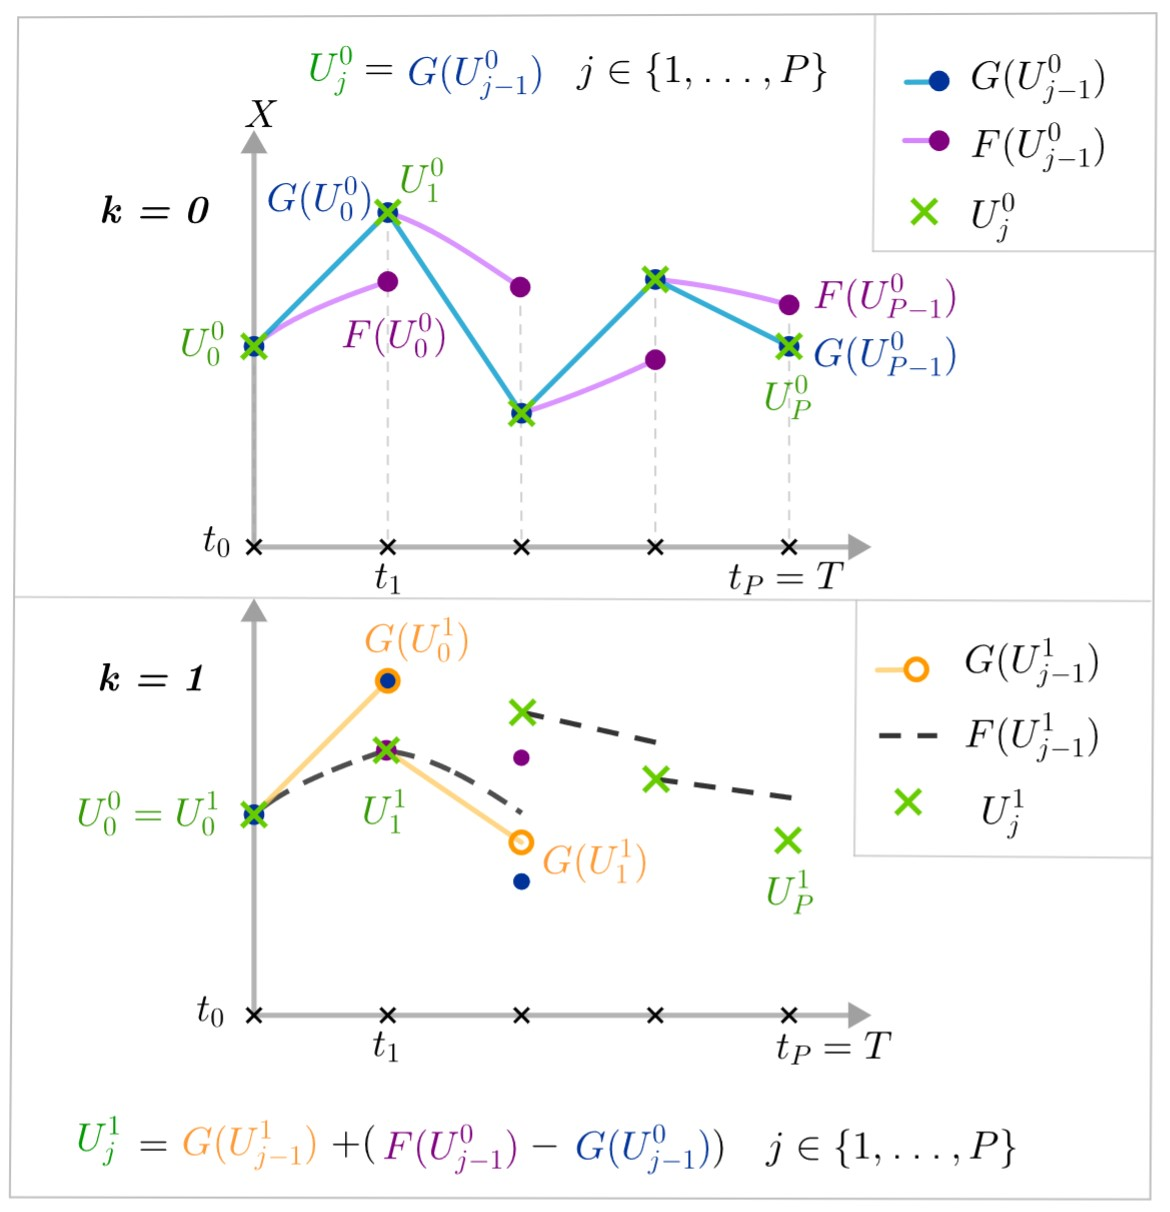
\includegraphics[width=\linewidth]{"images/parareal/parareal_6.jpg"}
				\captionof{figure}{ : Step 6}
				\label{parareal:6}
			\end{subfigure}
	\end{minipage}}
	\caption{Parareal method}
	\label{parareal}
\end{figure}

\subsubsection{Order of parareal method}

We say that the previous method is of order k (see \cite{partie2_ref2}) if there is a constant $c_k$ such that :
\begin{equation}
	\forall j\in\{0,\dots,P-1\} \qquad |U_j^k-U_{ex}(t_j)|+\max_{t\in[t_j,t_{j+1}]}|U_k(t)-U_{ex}(t)|\le c_k(\Delta t_G)^k
\end{equation}
where $U_j^k$ is the initial point at $t_j$ and iteration $k$, $U_{ex}(t_j)$ is the exact solution at the same time (at $t_j$ and iteration $k$), $U_k$ is the solution between $t_0$ and $T$ at iteration k and $U_{ex}$ is the exact solution between $t_0$ and $T$. Note that we calculate the maximum just between $t_j$ and $t_{j+1}$. \\

\noindent In the following, we will note : \quad $\mathcal{E}(j,k)=|U_j^k-U_{ex}(t_j)|+\max_{t\in[t_j,t_{j+1}]}|U_k(t)-U_{ex}(t)|$

\subsection{Application to the harmonic oscillator}

\noindent Before moving on to the Lorenz system, we will consider a mass-spring system of the following form :

\begin{equation}
	\frac{\partial^2 x}{\partial t^2}+\omega_0^2 x = 0 \quad \iff \quad \frac{\partial^2 x}{\partial t^2}=-\omega_0^2 x \quad \text{with} \quad \omega_0=\sqrt{\frac{k}{m}}.
	\label{osc}
\end{equation}

\noindent $k$ and $m$ are the spring stiffness and the suspended mass respectively. We are interested in this equation because its exact solution is known and is of the form :
$$x(t) = x_0 \cos(\omega_{0}t+\phi_0).$$

\noindent First of all, the numerical methods we have seen in Section \ref{sec4} (such as Runge Kutta order 4 in section \ref{sec4.4}), allow us to solve first order differential equations. But the harmonic oscillator equation (\ref{osc}) is a second order equation. We will therefore start by making a simple change of variable which will allow us to replace this second order differential equation by a system of two first order equations. We pose :
 
$$\qquad \frac{\partial x}{\partial t}=v \quad \Rightarrow \quad \frac{\partial^2 x}{\partial t^2}=\frac{\partial v}{\partial t}.$$

\noindent As a result the equation becomes :

$$\left\{\;\begin{aligned}
	\frac{\partial x}{\partial t}&=v \\
	\frac{\partial v}{\partial t}&=-\omega_0^2 x
\end{aligned}\right.
$$

\noindent Let's take an example to understand how we can determine the exact solution from the initial conditions that we will take. For example if we take $\omega_0=5$ and $(x(0),v(0))=(0,1)$, we have :

$$\left\{\;\begin{aligned}
	x(0)&=0 \\
	v(0)&=1
\end{aligned}\right. \quad \Rightarrow 
\left\{\;\begin{aligned}
	x_0 \cos(\phi_0)&=0 \\
	-x_0 \omega_{0} \sin(\phi_0)&=1
\end{aligned}\right.  \quad \Rightarrow  
\left\{\;\begin{aligned}
	x_0&=\frac{-1}{5} \\
	\phi_0&=\frac{\pi}{2}
\end{aligned}\right.
$$

\noindent And thus the solutions of the equation are of the form :

$$x(t) = \frac{-1}{5}\cos(5t+\frac{\pi}{2})$$

\noindent We want now to apply the parareal method on the harmonic oscillator. For the two integrators we will take Runge Kutta order 4 method with a small time step for $F$ and a larger one for $G$. With the previous example, we have the following parameters with 3 process :
$$x(0)=0,\quad v(0)=1, \quad\omega_0=5, \quad x_0=\frac{-1}{5}, \quad \phi_0=\frac{\pi}{2}$$
We then obtain the following results according to the iterations of the method :
\begin{figure}[H]
	\fbox{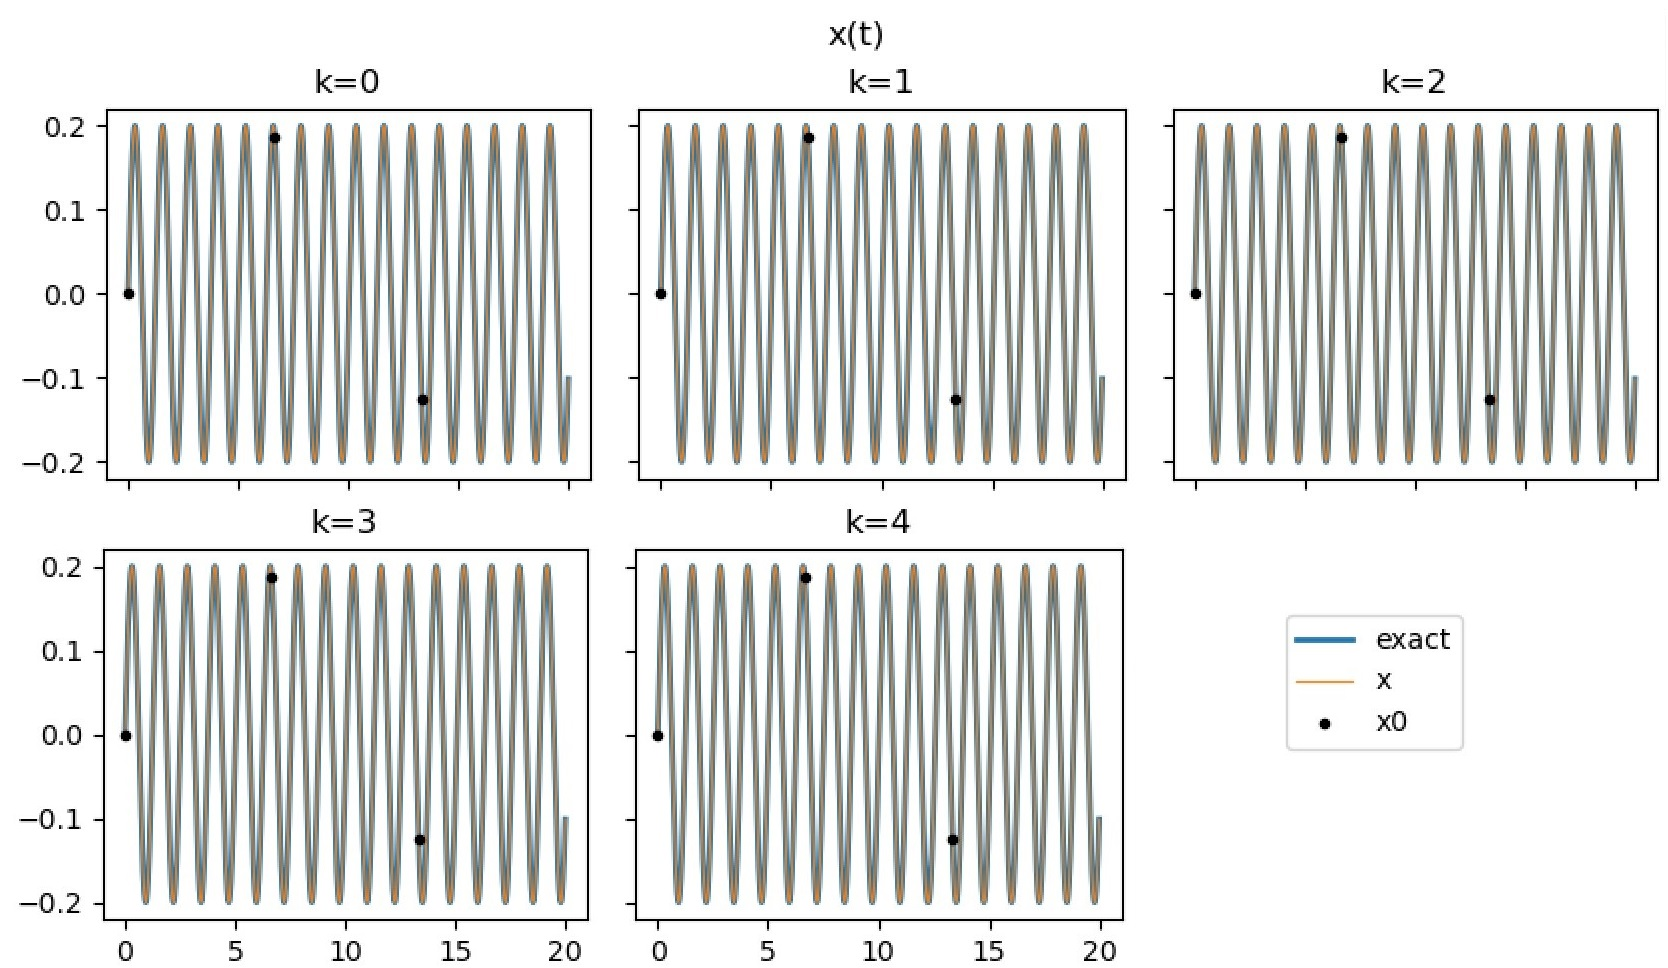
\includegraphics[width=\linewidth]{"images/parareal/osci_1.jpg"}}
	\caption{Plot of the exact solution and the approximate solution (for given parameters).}
\end{figure}
\noindent We see that the system seems to converge in 5 iterations, i.e. between the iterations $k=4$ and $k=5$ the points $U_n^k$ are equal to almost one $\epsilon$. \\

\noindent Let us now check the order of convergence of the method on this same example. In the following graph, the blue curve represents the maximum on $j$ of $\mathcal{E}(j,k)$ according to the iterations $k$ and the orange curve represents the $(\Delta t_G)^k$.
\begin{figure}[H]
	\centering
	\fbox{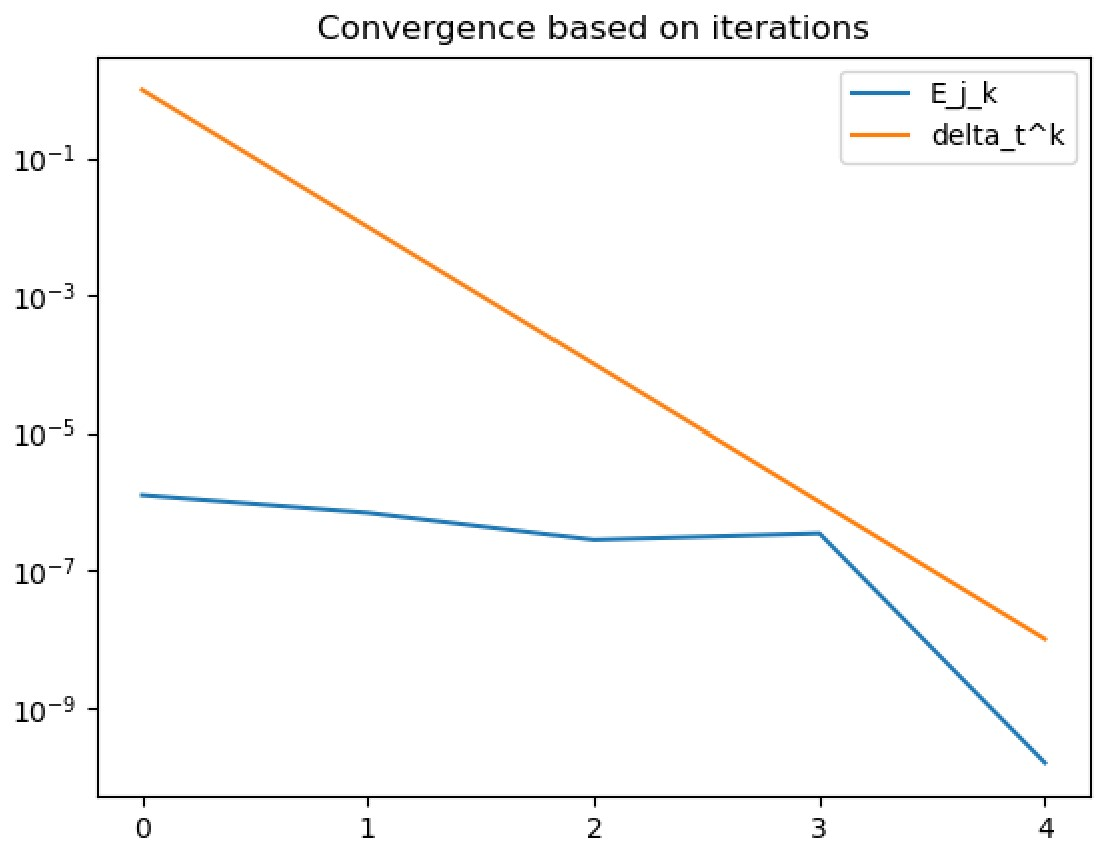
\includegraphics[width=0.4\linewidth]{"images/parareal/osci_cvg_1.jpg"}}
	\caption{Plot of $\mathcal{E}(j,k)$ and $(\Delta t_G)^k$.}
\end{figure}
\noindent We can see that the blue curve is below the orange curve for all the k iterations and so for the parameters fixed previously on the oscillator, the method is of order k.

\subsection{Application to the Lorenz system}

We want now to apply the parareal method on the Lorenz system. In the previous explanation, we have also :

$$X'=\begin{pmatrix}
    x' \\
    y' \\
    z'
\end{pmatrix}, \quad X=\begin{pmatrix}
    x \\
    y \\
    z
\end{pmatrix} \quad and \quad f(t,X)=\begin{pmatrix}
    \sigma(y-x) \\
    x(r-z)-y \\
    xy-bz
\end{pmatrix}.$$

\noindent For the two integrators we will take Runge Kutta order 4 method with a small time step for $F$ and a larger one for $G$. \\

\noindent We choose the following parameters :
$$\sigma=10, \quad b=\frac{8}{3}, \quad r=28, \quad X_0=(5,5,5), \quad t_0=0.$$

\noindent For this choice of parameters, we have a butterfly wing pattern (see Figure \ref{lorenz:exact3D}) and we have the three following curves (see Figure \ref{lorenz:exact}) for the representation of the 3 variables x, y and z as functions of time.

\begin{figure}[H]       
	\begin{minipage}[t]{0.48\linewidth}
		\centering
		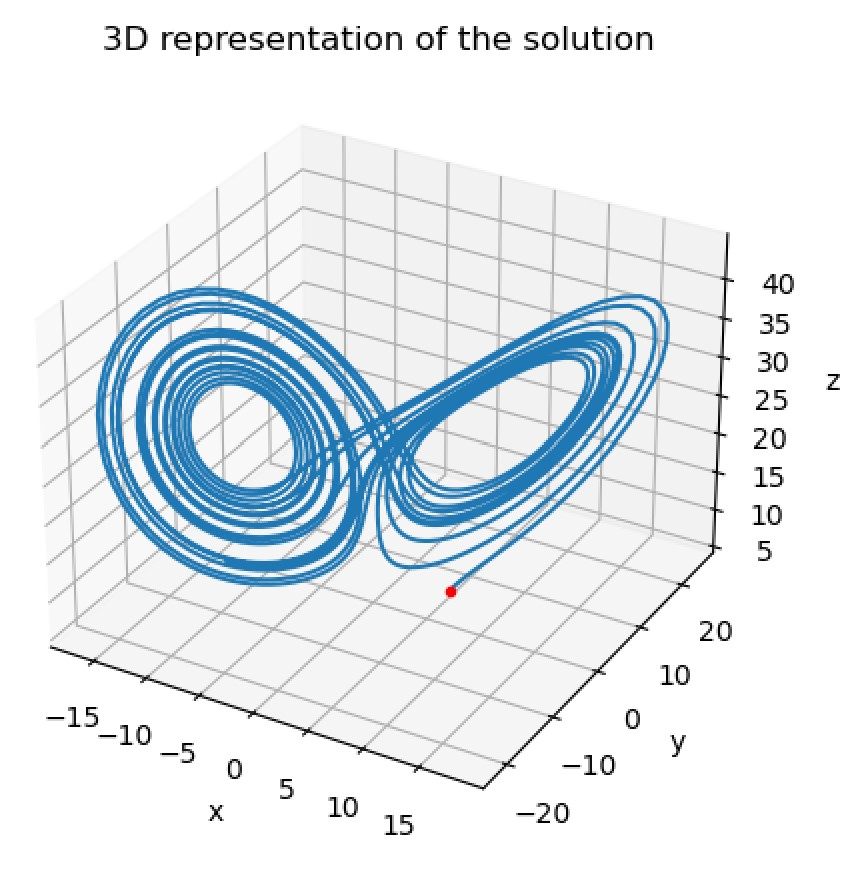
\includegraphics[width=\linewidth]{"images/parareal/lorenz_exact_3D.jpg"}
	\end{minipage} \hfill
	\begin{minipage}[t]{0.48\linewidth}
		\centering
		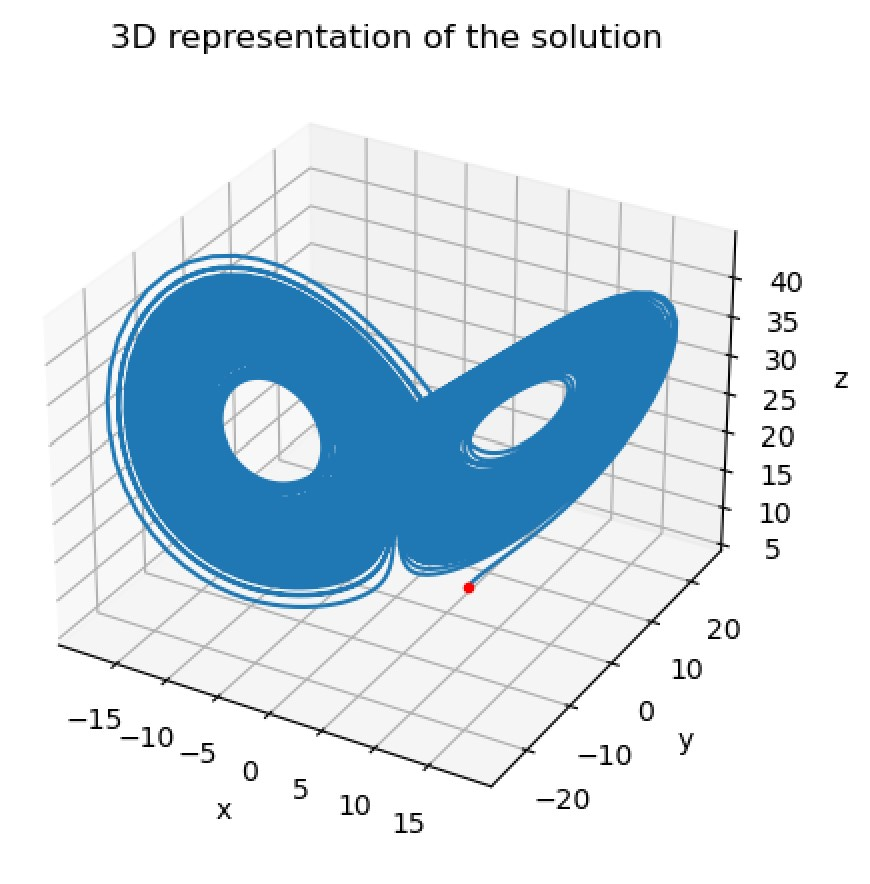
\includegraphics[width=\linewidth]{"images/parareal/lorenz_exact_3D_T200.jpg"}
	\end{minipage}
	\captionof{figure}{Solution 3D of the Lorenz system with given parameters ($T=20$ and $T=200$)}
	\label{lorenz:exact3D}
\end{figure}

\begin{figure}[H]  
	\centering     
	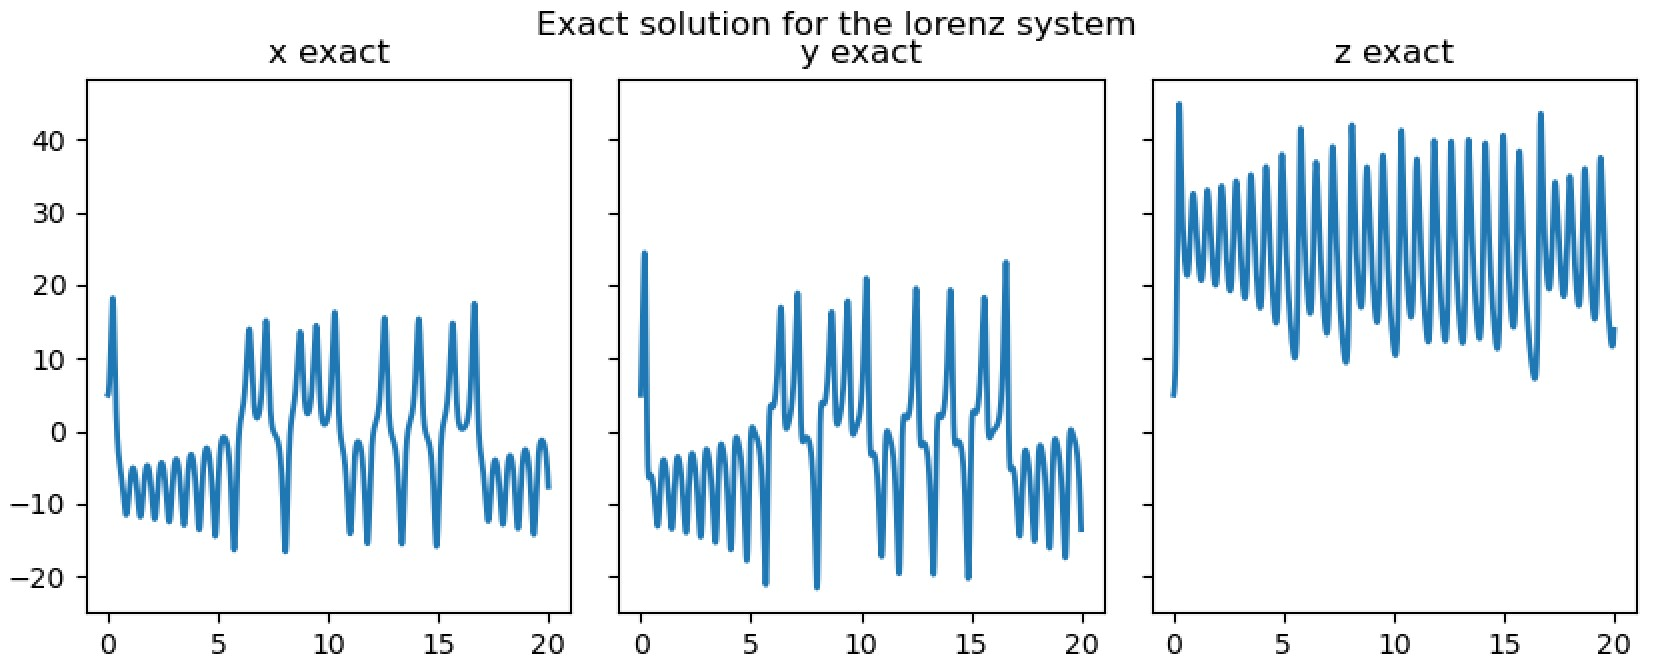
\includegraphics[width=\linewidth]{"images/parareal/lorenz_exact.jpg"}
	\captionof{figure}{Solution of the Lorenz system with given parameters}
	\label{lorenz:exact}
\end{figure}

\noindent We will now apply the parareal method (from $t_0=0$ to $T=20$) with the previous parameters for different numbers of processes (from 1 to 4 processes : see Figures \ref{lorenz:1}, \ref{lorenz:2}, \ref{lorenz:3} and \ref{lorenz:4}). We are going to be interested here only in the variable x.

\begin{enumerate}[label=\textbullet]

	\item With 1 process we see (as explained in the "Remarks" of the section \ref{section parareal method}) that there are only two iterations and that they are similar (because they start from the same initial point and there is no other initial point).
	\begin{figure}[H]
		\centering       
		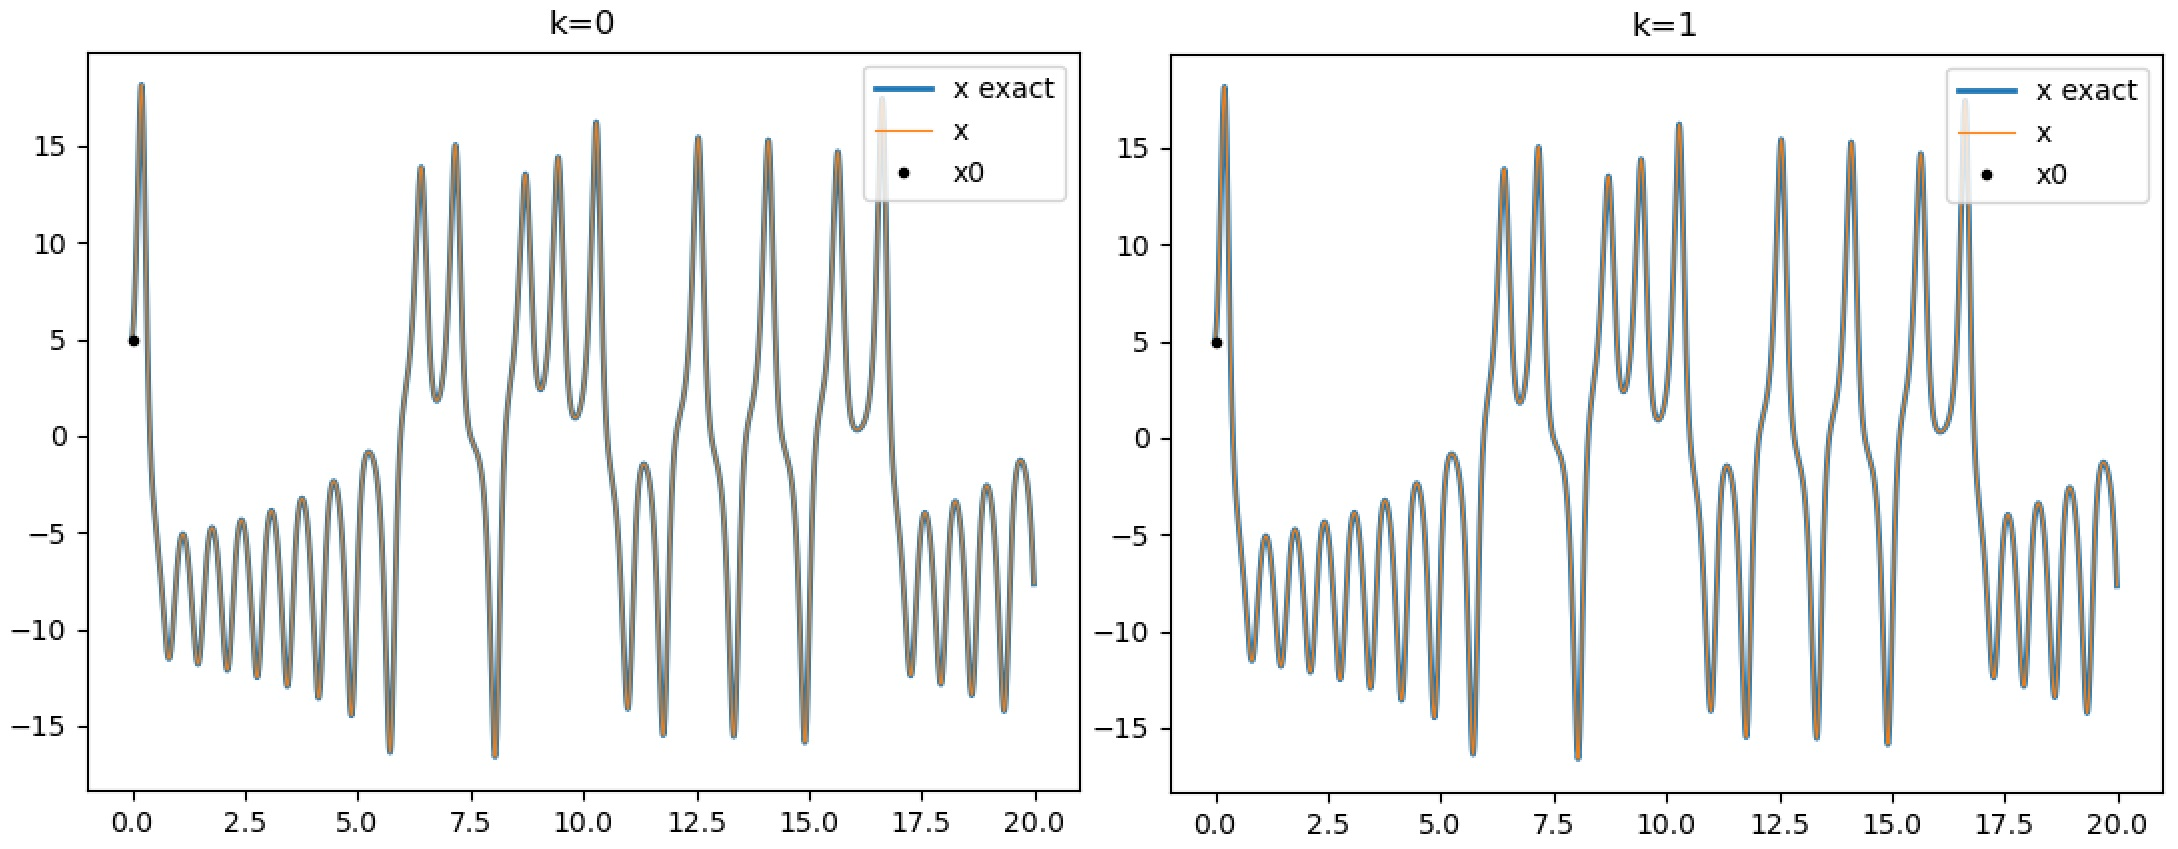
\includegraphics[width=0.9\linewidth]{"images/parareal/lorenz_1p.jpg"}
		\captionof{figure}{Parareal method on the Lorenz system with 1 process}
		\label{lorenz:1}
	\end{figure}
\newpage
	\item With two processes we see that the solution converges in 3 iterations.
	\begin{figure}[H]       
		\centering
		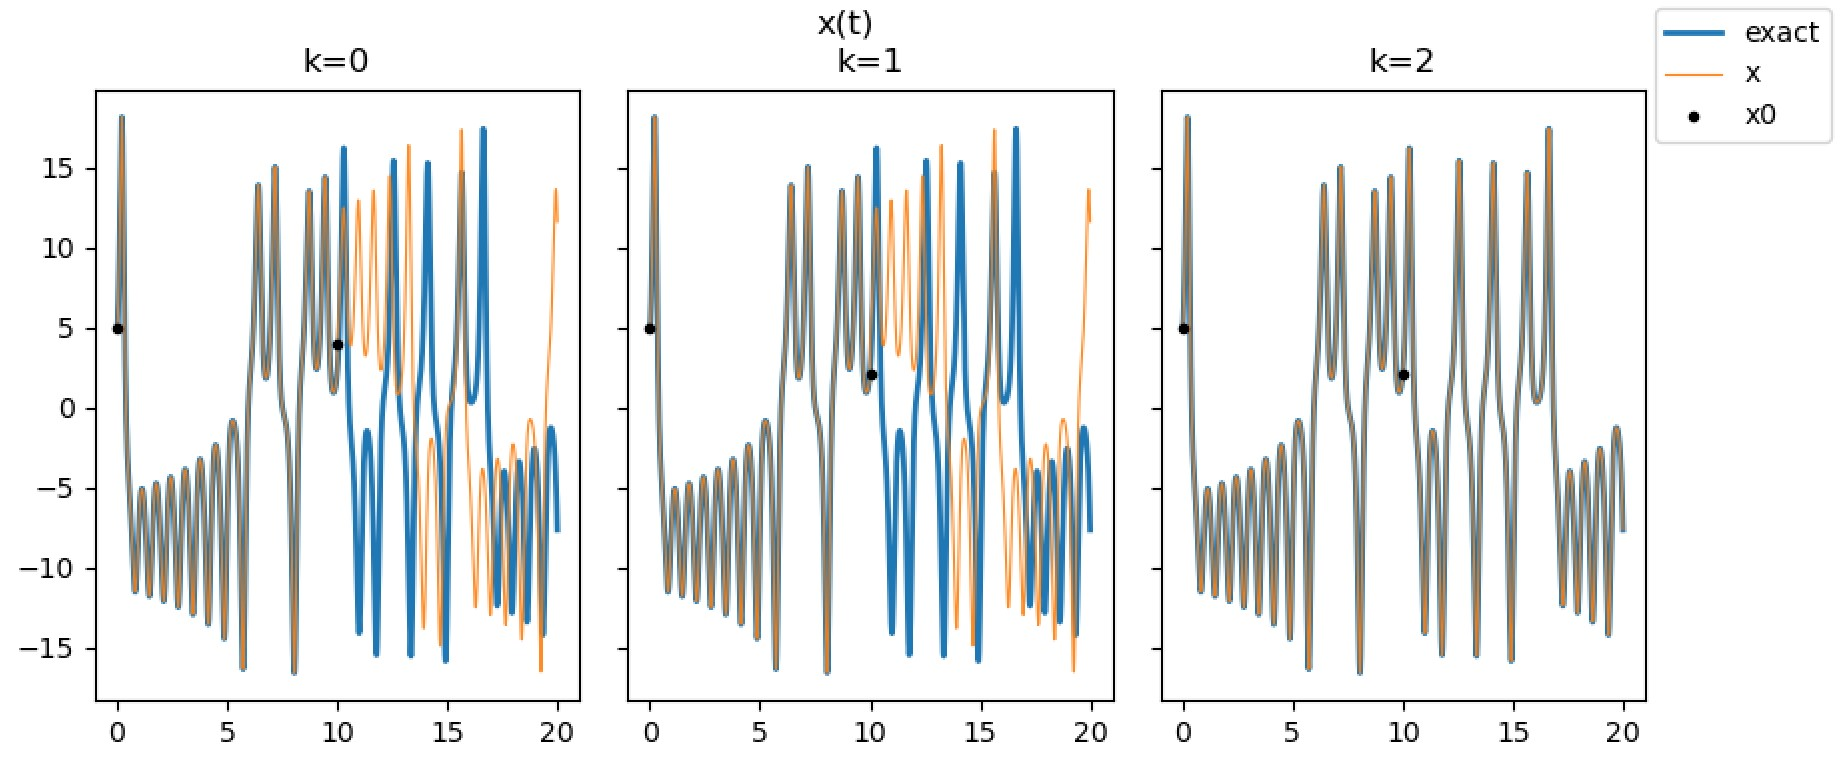
\includegraphics[width=0.9\linewidth]{"images/parareal/lorenz_2p.jpg"}
		\captionof{figure}{Parareal method on the Lorenz system with 2 processes}
		\label{lorenz:2}
	\end{figure}
	\item With three processes we see that the solution converges in 5 iterations.
	\begin{figure}[H]       
		\centering
		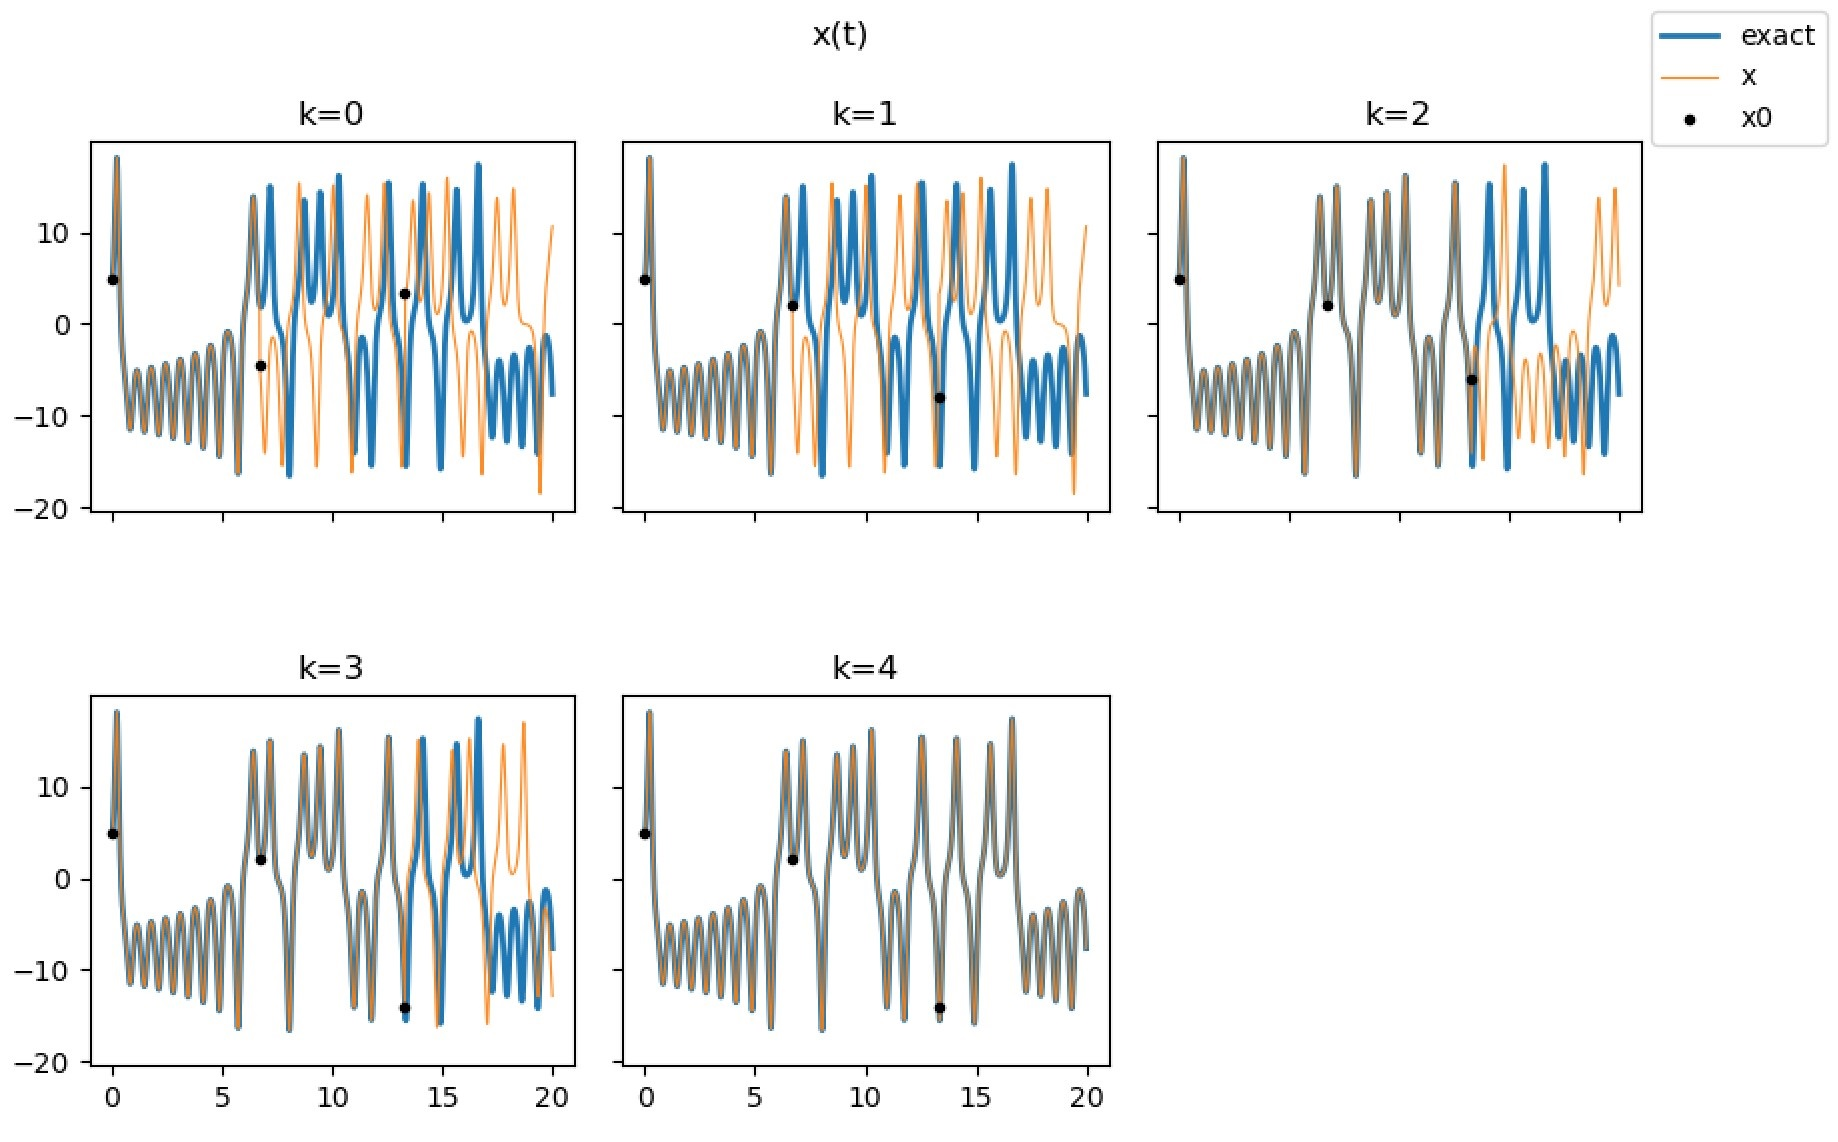
\includegraphics[width=0.9\linewidth]{"images/parareal/lorenz_3p.jpg"}
		\captionof{figure}{Parareal method on the Lorenz system with 3 processes}
		\label{lorenz:3}
	\end{figure}
\newpage
	\item With four processes we see that the solution converges in 7 iterations.
	\begin{figure}[H]       
		\centering
		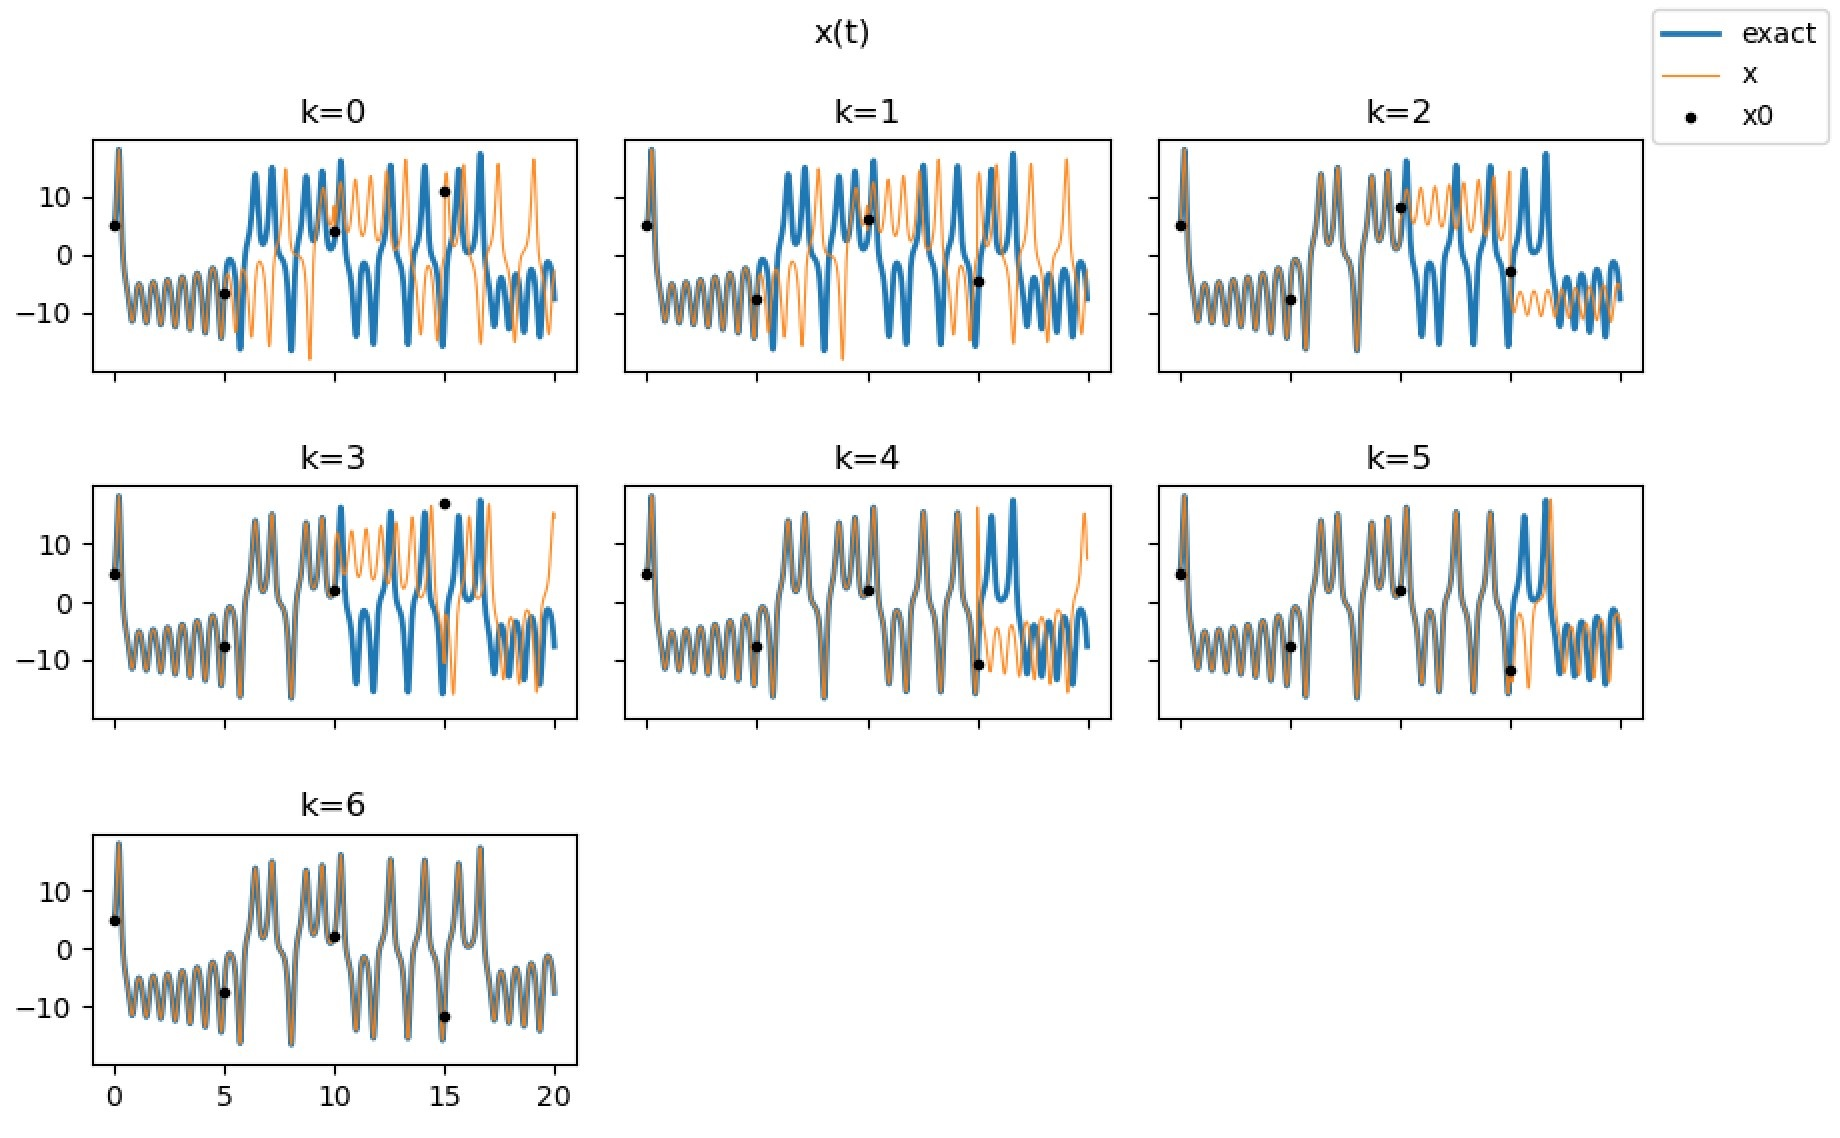
\includegraphics[width=0.9\linewidth]{"images/parareal/lorenz_4p.jpg"}
		\captionof{figure}{Parareal method on the Lorenz system with 4 processes}
		\label{lorenz:4}
	\end{figure}

\end{enumerate}

\noindent According to the results, it seems that that as we increase the number of processes, the number of iterations increases. We can therefore wonder why the parareal method is efficient. The table below (Table \ref{time})  contains the execution time first of the iterative method with RK4 (the sequential method) and the execution time for different numbers of processes (parareal method) and this for various fine and coarse time steps.

\begin{table}[H]
	\centering
	\begin{tabular}{| c || c | c | c | c | c |}
		\hline
		\multirow{2}{1.5 cm}{$\Delta t$} & \multirow{2}{1.5 cm}{Seq} & \multirow{2}{1.5 cm}{1 proc} & \multirow{2}{1.5 cm}{2 proc} & \multirow{2}{1.5 cm}{3 proc} &\multirow{2}{1.5 cm}{4 proc} \\
		& & & & & \\
		\hline 
		F : 0.0025 & \multirow{2}{1.5 cm}{30s} & \multirow{2}{1.5 cm}{36s} & \multirow{2}{1.5 cm}{10s} & \multirow{2}{1.5 cm}{9,7s} & \multirow{2}{1.5 cm}{9,4s} \\
		G : 0.025 & & & & & \\
		\hline 
		F : 0.00125 & \multirow{2}{1.5 cm}{1m19} & \multirow{2}{1.5 cm}{1m42} & \multirow{2}{1.5 cm}{39s} & \multirow{2}{1.5 cm}{32s} & \multirow{2}{1.5 cm}{29s} \\
		G : 0.0125 & & & & & \\
		\hline 
		F : 0.001 & \multirow{2}{1.5 cm}{1m52} & \multirow{2}{1.5 cm}{3m40} & \multirow{2}{1.5 cm}{1m56} & \multirow{2}{1.5 cm}{1m29} & \multirow{2}{1.5 cm}{1m16} \\
		G : 0.01 & & & & & \\	 
		\hline
	\end{tabular}
	\caption{Execution time for various time steps ($T=200$).}
	\label{time}
\end{table}

\noindent \underline{\textit{Observations :}} 

\begin{itemize}[label=-]
	\item It seems that the time in sequential and with the parareal method with 1 process is not the same. Moreover for the different steps calculated, we have that the execution time with 1 process is greater than for the sequential method. This can be explained by 2 main things. First of all, we have seen previously that there are necessarily 2 iterations which are done on $[t_0,T]$ contrary to the sequential method where there is only one. This problem is easily solved if we compute only the fine and coarse solutions at the first iteration (because the point $U_0^k$ is identical for all k). Thereafter, the parareal method also computes the coarse solution which is not needed at all and is not computed sequentially.
	\item It seems that the time for the parareal method with $P$ processes is not the time of the sequential method divided by $P$. It seems obvious that (with intervals of the same length for each process), the time for the parareal method is only divided by P if there is only one iteration, which is never the case.
	\item It seems that if we increase the number of processes, the time does not necessarily decrease (as between $P=3$ and $P=4$ for $\Delta t_F=0.001$ and $\Delta t_G=0.01$), so we have to find the right balance between the parameters $\Delta t_F$, $\Delta t_G$, $[t_0,T]$ and $P$.
\end{itemize}

\noindent \underline{\textit{Remarks :}} Improvement of the parareal method implementation 

\begin{itemize}[label=-]
	\item A first improvement for the implementation of the method could be to make a separate case for $P=1$. For this case, we would only compute the fine solution once on $[t_0,T]$.
	\item As said before, one possibility to improve the permorfances would be to compute only the fine and coarse solutions between $t_0$ and $t_1$ at the first iteration because they are the only ones that never change during the iterations. 
	\item In the same way, we could never compute the coarse solution between $t_{P-1}$ and $t_P$ because we never use it and we can compute the fine solution on this interval only at the last iteration (i.e. when the solution converges) because we need this information only to obtain the final solution of the system.
\end{itemize}

\noindent \underline{\textit{Future of the project :}}

\begin{itemize}[label=-]
	\item The first thing that could be done in the future of this project would be to implement the remarks (Improvement of the parareal method implementation) made earlier.
	\item Then, we could try to understand why there seems to be a "stagnation" in the execution times and try to find a way to choose a number of processes $P$ which is optimal (the fastest) according to the parameters we have.
	\item We could also see what happens if we take a lot more intervals that are spread over the different processes. Because here we are limited as the number of processes is equal to the number of intervals. Would we have an improvement for the speed of the method or on the contrary, would we have many more iterations because the initial points would be much less precise?
\end{itemize}